\documentclass[a4paper,12pt]{scrartcl} 
\usepackage{ulem}
\usepackage{graphicx}
\usepackage{amsmath}
\usepackage[warn]{mathtext} 
\usepackage[T2A]{fontenc} 
\usepackage[utf8]{inputenc}
\usepackage[english]{babel} 
\usepackage{indentfirst} 
\usepackage{misccorr} 
\usepackage{caption}
\usepackage{graphicx}
\usepackage{subcaption}
\usepackage{xcolor}
\usepackage{wrapfig}
\usepackage{algorithm}
\usepackage{algpseudocode}
\captionsetup{compatibility=false}
\begin{document}

\title{SyntenyFinder: A Synteny Blocks Generation and Genome Comparison Tool}
\author{Intern: Ilya Minkin\\
	Advisor: Son Pham}
\date{}
\maketitle

\begin{abstract}
We present algorithm for finding synteny blocks in genomes represented as nucleotide sequences. The algorithm is based
on colored De Bruijn graphs and graph simplifications. Our method is able to reconstruct synteny blocks previously found
by ad hoc methods.
\end{abstract}

\section{Introduction}

Recent growth of number of sequenced genomes arises question about their evolution relationship. 
In order to perform rearrangement analysis, the genomes must be decomposed into conservative segments,
called synteny blocks. Currently existing tools for solving this problem, like DRIMM-Synteny
\cite{Pham2010}, require the genomes to be presented as sequences of enumerated local alignments, or \textit{anchors}.
Usually, anchors represent homologous genes. At this moment, there are no general purpose tools that can
find synteny blocks from the genomes represented as unannotated nucleotide sequences.

De Bruijn graphs are extensively used in bioinformatics for genome assembly \cite{Pevzner2001, Iqbal2012}. 
In this work we address problem of finding synteny blocks from nucleotide sequences. We propose new 
algorithm for this task based on colored De Bruijn graph.


\section{Problem definition}

Suppose that we are given a set \(S = \lbrace s_{1}, s_{2}, \ldots, s_{n} \rbrace \) of chromosomes, and each
chromosome is represented as a string over alphabet \(\lbrace A, C, G, T \rbrace \). The task of finding synteny
blocks is to find a set of so called conserved regions \(C = \lbrace C_{1}, C_{2}, \ldots , C_{n} \rbrace \), where
each conserved region \(C_{i}\) is a set of substrings of chromosomes from \(S\). Such regions are supposed 
to cover most of the genome for closely related species.  All substrings forming a conserved region \(C_{i}\) must be
 "similar" to each other according to some criterion of similarity. Note that problem of finding synteny blocks in a set
of chromosomes is equivalent to a problem of finding synteny blocks in one "superchromosome" obtained from
concatenating all chromosomes from the set.
At this moment there is no generally accepted formal criterion of similarity exist, so the problem of finding synteny blocks is ill-defined.

In our work we introduce new criterion of similarity based on De Bruijn graphs and graph simplifications.

\section{General idea}

\begin{figure}
        \begin{subfigure}[a]{1\textwidth}
		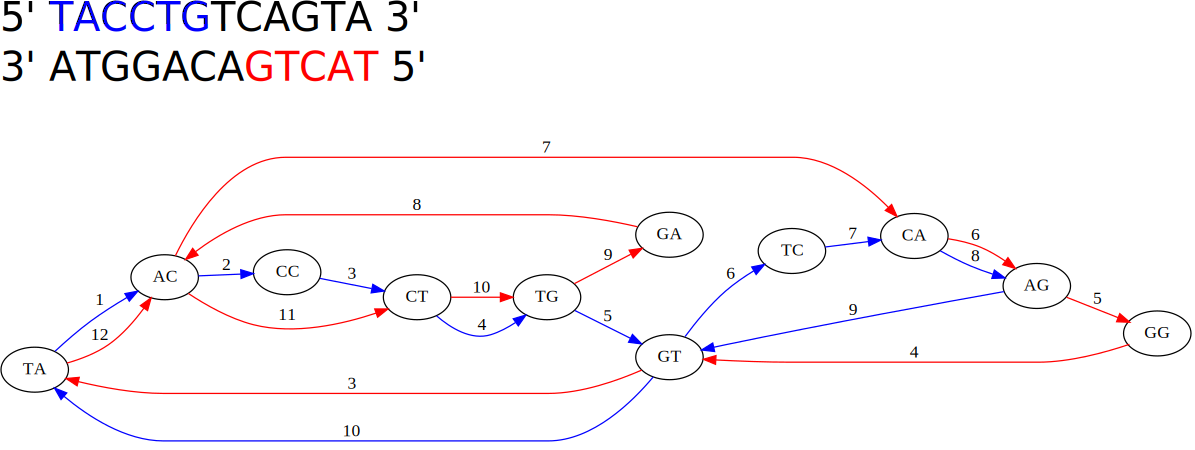
\includegraphics[scale = 0.50]{graph1.pdf}
		\small \caption{De Bruijn graph built from string \("acgcattgtactcatt"\) and \(k = 2\). Non-branching paths correspond to multiple
			copies of the same substrings.}
		\label{DeBruijnA}
        \end{subfigure}
	\\
        \begin{subfigure}[b]{1\textwidth}
		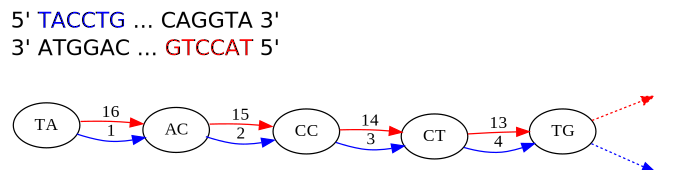
\includegraphics[scale = 0.50]{graph2.pdf}
		\small \caption{Same De Bruijn graph after simplification. Replacing \("acGca"\) by \("acTca"\) we obtain long non-branching path
			that corresponds to the synteny block.}
		\label{DeBruijnB}
        \end{subfigure}
	\small \caption{Illustration of De Bruijn graphs and graph simplification}
\end{figure}

Informally speaking, \(k\)-dimensional De Bruijn graph is a graph with vertices representing all possible strings of length \(k\)
(called \(k\)-mers). In this graph two vertices \(u\) and \(v\) are connected by a oriented edge from \(u\) to \(v\) if exists
\((k + 1)\)-mer \(w\) such that \(u\) is the prefix of \(w\) and \(v\) is the suffix of \(w\).

Given  a number \(k\) and a string \(S\) we can build De Bruijn \(G\) graph from the string as follows: for each \((k + 1)\)-mer found 
in \(S\) we add corresponding edge to \(k\)-dimensional De Bruijn graph and label it with position of first symbol belonging to
the \((k + 1)\)-mer (multiedges with different labels are allowed). In this graph we allow only paths that have consecutive labels
on edges. It is easy to see that with such restriction every substring of \(S\) corresponds to a valid path in \(G\). Example of such
De Bruijn graph built from the string \(S = "acgcattgtactcatt" \) and \(k = 2\) is depicted on Figure~\ref{DeBruijnA}.

Note that two copies of substring \("catt"\) form non-branching path consisting of edges with multiplicity \(2\) in this graph. Single
mismatch in substrings \("acGca"\) and \("acTca"\) form so-called "bulge", unoriented cycle generated by two valid paths with
coinciding ends. If we replace one branch of the bulge by another (say, replace \("acGca"\) by \("acTca"\)) then we will obtain
long non-branching path (Figure~\ref{DeBruijnB}).

This heuristic forms basis of our method -- conserved regions in different parts of the genome contain conserved basepairs, but
such regions are disrupted by indels and mismatches. These artifacts generate bulges in the graph that spoil non-branching paths.
We remove bulges having size less than some predefined constant and thus obtain non-branching paths corresponding to the
conserved regions. The process of removing from the graph bulges is called \textit{simplification}.

Conserved regions can be located on opposite strands of DNA. To handle this, we use \textit{colored} De Bruijn graphs \cite{Iqbal2012}.
Given string \(S\), for each \((k + 1)\)-mer found in \(S\) we add corresponding edge to the graph and color it \textit{blue}, for 
each \((k + 1)\)-mer found in reverse-complementary counterpart of \(S\) we add corresponding edge to the graph and color it \textit{red}.
In this graph, coinciding paths with different colors represent synteny blocks located on opposite strands of DNA.

Our algorithm depends on two parameters -- \(k\) and minimum allowed size of a bulge. It is reasonable to use as high \(k\) as possible
to keep graph structure simple and avoid connecting regions that are actually not homologous. But even highly conserved regions can
lack shared \(k\)-mers for \(k > 30\). To overcome this, we first find a set of local alignments in the genome (by BLAST), then substitute
one aligned subsequence by another for each found significant local alignment. So the pipeline is following:\\
1) Find all alignments in the genome(s) and perform substitution (see above) \\
2) Build De Bruijn graph \\
3) Simplify the graph \\
4) Output synteny blocks as non-branching path in the graph 

\section{Detailed description}

In this section we will present our algorithm in more formal fashion. Suppose that we are given a string \(S = (s_{0}, s_{1}, \ldots, s_{n - 1})\)
over alphabet \(\Sigma = \lbrace A, C, G, T \rbrace\), two numbers \(k\) and \(\delta\). We denote by \(S(i, j)\) the \((i, j)\) substring of S,
\(S(i, j) = (s_{i}, s_{i + 1}, \ldots, s_{j}) \).  Let's denote by \(\bar{S}\) string that is the reverse complementary of \(S\). 

Colored De Bruijn graph is graph \(G_{k} = (V, E) \) where \(V = \Sigma ^ k \). We define three functions: \\
1) \(Pos : \, E \rightarrow \mathbb{N} \) \\
2) \(Spell : \, E \rightarrow \Sigma ^ {k + 1} \) \\
3) \(Color : \, E \rightarrow \lbrace Blue, Red \rbrace \) 

For each \(i \in \lbrace{0, 1, \ldots, n - k - 1} \rbrace \) we add two oriented edges to the graph: \\
1) \(e = (S(i, i + k - 1), S(i + 1, i + k)), \, Color(e) = Blue, \, Pos(e) = i, \, Spell(e) = S(i, i + k) \) \\
2) \(\bar{e} = (\bar{S}(i, i + k - 1), \bar{S}(i + 1, i + k)), \, Color(\bar{e}) = Red, \, Pos(\bar{e}) = i, \, Spell(\bar{e}) = \bar{S}(i, i + k) \)

A path in \(G_{k}\) is a sequence of edges \(P = (e_{1}, e_{2}, \ldots, e_{n})\) iff \(Pos(e_{i+1})  = Pos(e_{i}) + 1\) and
\(Color(e_{i + 1}) = Color(e_{i})\). Let's denote by \(Start(P)\) first vertex of the path \(P\) and by \(End(P)\) the last vertex of \(P\).

\newpage

A pair of paths \(B =\lbrace b_{1}, b_{2} \rbrace \)
is called a \textit{bulge}, iff following holds: \\
1) \(|b_{1}| < \delta\ \wedge |b_{2}| < \delta\) \\
2) \(Start(b_{1}) = Start(b_{2}) \wedge End(b_{1}) = End(b_{2}) \) \\
3) \(b_{1}\) and \(b_{2}\) have no common vertices except \(Start(b_{1})\) and \(End(b_{1})\) \\
4) There are no edges \(e_{1} \in b_{1}, e_{2} \in b_{2} \) such that \(Spell(e_{1}) = Spell(e_{2})\)

A vertex \(v\) is called \textit{bifurcation} iff there are at least two outgoing (ingoing) edges \(e_{1}, e_{2}\) 
from (to) \(v\) such that \(Spell(e_{1}) \neq Spell(e_{2})\). A set of paths \(P_{nb} = \lbrace P_{1}, P_{2}, \ldots, P_{n} \rbrace\)
is said to form a \textit{non-branching path} iff \(|P_{1}| = |P_{2}| = \ldots |P_{n}| \) and \(Spell(e_{i, k}) = Spell(e_{j, k}) \),
where \(e_{i, j}\) denote \(j\)-th edge in the \(i\)-th path, i.e. all paths spell the same substring.

\begin{figure}
	\includegraphics[scale = 0.50]{graph3.pdf}
	\small \caption{Colored De Bruijn graph for string \(S = "acctgtcagt" \) }
	\label{ColoredDeBruijn}
\end{figure}

Let's illustrate above definitions on a simple example. Colored De Bruijn graph built from string \(S = "acctgtcagt"\)
is depicted on Figure~\ref{ColoredDeBruijn}. Here \(\bar{S} = "actgacaggt"\). Vertices \("ac", "ct", "tg"\) are 
bifurcations, while \("cc", "tc", "ga"\) are not. Two paths \(("ac", "ct")\) and \((("ac", "cc"), ("cc", "ct"))\) form a bulge.
Two multiedges \(("ct", "tg")\) form a non-branching path.

\section{Experimental results}
Results
\section{Conclusion}
Conclusion

\begin{thebibliography}{9}
\bibitem{Pham2010}
	Son K. Pham, Pavel A. Pevzner.
	DRIMM-Synteny: decomposing genomes into evolutionary conserved segments.
	Bioinformatics (2010)  26  (20):  2509-2516.
\bibitem{Pevzner2001}
	Pavel A. Pevzner, Haixu Tang, Michael S. Waterman.
	An Eulerian path approach to DNA fragment assembly.
	Proc. Natl. Acad. Sci. USA. 2001 Aug 14; 98(17): 9748-53.
\bibitem{Iqbal2012}	
	Zamin Iqbal, Mario Caccamo, Isaac Turner, Paul Flicek, McVean.
	De novo assembly and genotyping of variants using colored de Bruijn graphs.
	Nat Genet. 2012 Jan 8;44(2):226-32. doi: 10.1038/ng.1028.
\bibitem{Kellis2004}
	Manolis Kellis, Bruce W. Birren, Eric S. Lander.
	Proof and evolutionary analysis of ancient genome duplication in the yeast Saccharomyces cerevisiae.
	Nature 2004 Apr 8;428 (6983): 617-24.
\end{thebibliography}

\end{document}